\documentclass{article}

\usepackage{blindtext}
\usepackage{graphicx}
\usepackage{wrapfig}
\usepackage[skip=1ex]{caption}
\usepackage{subcaption}
\usepackage{mdframed}
\usepackage{amsmath}
\usepackage{amsfonts}
\usepackage{amssymb}
\usepackage{amstext}
\usepackage{cancel}
\usepackage{enumitem}
\usepackage[english]{babel}
\usepackage{helvet}
\usepackage{microtype}
\usepackage[pdftex]{hyperref}
\usepackage{float}
\usepackage{nicematrix}
\usepackage{xcolor}
\usepackage{tikz}
\usepackage{geometry}
\geometry{
    a4paper,
    left=2cm,
    right=2cm,
    top=1cm,
    bottom=1cm
}

\special{papersize=8.5in,11in}
\setlength{\pdfpageheight}{\paperheight}
\setlength{\pdfpagewidth}{\paperwidth}

% Macros

% Make inline frac bigger
\newcommand\ifrac[2]{{\displaystyle\frac{#1}{#2}}}

% Definitions
\def\wstar{\overset{*}{\rightharpoonup}}
\def\grad{\nabla}
\def\nt{\notag}
\def\dt{\partial_t}
\def\hal{\frac{1}{2}}
\def\ep{\varepsilon}
\def\cK{\mathcal{K}}
\def\cA{\mathcal{A}}
\def\cS{\mathcal{S}}
\def\Q{\mathbb{Q}}
\def\R{\mathbb{R}}
\def\Z{\mathbb{Z}}



\begin{document}



\title{Written Assignment 1}

\author{Niraj Venkat}

\date{}

\maketitle

\vspace{.8cm}
\boxed{\text{Exercise} \quad 1}\\\\

\begin{enumerate}[label=(\alph*)]
    \item
    \begin{align}
        v \wedge w  &= (e_1 + 2e_2) \wedge (e_2 + 2e_3) \tag*{\bfseries(Distributivity over addition)}\\
                    &= (e_1 \wedge e_2) \, + \,  2(e_1 \wedge e_3) \, + \, \cancelto{0}{2(e_2 \wedge e_2)} \, + \, 4(e_2 \wedge e_3) \notag\\
                    &= (e_1 \wedge e_2) \, + \,  2(e_1 \wedge e_3) \, + \, 4(e_2 \wedge e_3) \notag
    \end{align}

    \item 
    \begin{align}
        w \wedge v  &= -(v \wedge w) \tag*{\bfseries(Antisymmetric property)}\\
                    &= -(e_1 \wedge e_2) \, - \,  2(e_1 \wedge e_3) \, - \, 4(e_2 \wedge e_3) \notag
    \end{align}
    \item 
    \begin{align}
        v \wedge v  = 0 \notag
    \end{align}
\end{enumerate}



\vspace{1.8cm}
\boxed{\text{Exercise} \quad 2}\\\\

The result is a zero 3-vector.
\begin{align}
    \alpha_0 \wedge \alpha_1 \wedge \alpha_2 &= (e_1 + e_2) \wedge (e_1 + 2e_2) \wedge (e_1 + 4e_2) \notag\\
        &= ((e_1 \wedge e_1) + 2(e_1 \wedge e_2) + (e_2 \wedge e_1) + 2(e_2 \wedge e_2)) \wedge (e_1 + 4e_2) \notag\\    
        &= (\cancelto{0}{(e_1 \wedge e_1)} + 2(e_1 \wedge e_2) - (e_1 \wedge e_2) + \cancelto{0}{2(e_2 \wedge e_2)}) \wedge (e_1 + 4e_2) \notag\\
        &= e_1 \wedge e_2 \wedge (e_1 + 4e_2) \notag\\
        &= (e_1 \wedge e_2 \wedge e_1) + 4(e_1 \wedge e_2 \wedge e_2) \tag*{\bfseries(Antisymmetric property)}\\
        &= 0 \notag
\end{align}


\vspace{1.8cm}
\boxed{\text{Exercise} \quad 3}\\\\

Starting with 1-vectors $u, v \in \mathbb{R}^3$:
$$u \wedge v = -2(e_1 \wedge e_2) + 2(e_2 \wedge e_3)$$ which is a 2-vector in $\mathbb{R}^3$.\\
$$u \times v = 2e_1 -2e_3$$ which is a 1-vector in $\mathbb{R}^3$.


\vspace{1.8cm}
\boxed{\text{Exercise} \quad 4}\\\\

\begin{enumerate}[label=(\alph*)]
    \item
    \begin{align}
        u \wedge v + v \wedge w &= u \wedge v - w \wedge v = (u - w) \wedge v \tag*{\bfseries(Distributivity)}\\
            &= (e_1+e_2-e_3-3e_1-e_2) \wedge (e_1-e_2+2e_3) \notag\\
            &= 2(e_1 \wedge e_2) -3(e_1 \wedge e_3) - (e_2 \wedge e_3) \notag
    \end{align}
    \item
    \begin{align}
        u \wedge v \wedge w &= (e_1+e_2-e_3) \wedge (e_1-e_2+2e_3) \wedge (3e_1+e_2) \tag*{\bfseries(Skipping zero terms)}\\
            &= \bigl[ -2(e_1 \wedge e_2) + 3(e_1 \wedge e_3) +3(e_2 \wedge e_3) \bigr] \wedge (3e_1+e_2) \notag\\
            &= 3(e_2 \wedge e_3 \wedge e_1) + 3(e_1 \wedge e_3 \wedge e_2) \notag\\
            &= 3(e_2 \wedge e_3 \wedge e_1) - 3(e_2 \wedge e_3 \wedge e_1) \notag\\
            &= 0 \notag
    \end{align}
\end{enumerate}



\vspace{1.8cm}
\boxed{\text{Exercise} \quad 5}\\\\


\begin{enumerate}[label=(\alph*)]
    \item $\star e_1 = e_2$
    \item $\star e_1 = e_2 \wedge e_3$
    \item Hodge star of $k-$vector is an $(n-k)-$vector.\\
    In $\mathbb{R}^2: \quad n = 2, \, k = 1$ so $\star e_1$ is a 1-vector.\\
    In $\mathbb{R}^3: \quad n = 3, \, k = 1$ so $\star e_1$ is a 2-vector.
\end{enumerate}


\vspace{1.8cm}
\boxed{\text{Exercise} \quad 6}\\\\


\begin{enumerate}[label=(\alph*)]
    \item
    \begin{align}
        \star \alpha &= \star(e_1 + e_2 + e_3) \tag*{\bfseries(Distributivity over addition)}\\
            &= \star e_1 + \star e_2 + \star e_3 \notag\\
            &= (e_2 \wedge e_3) + (e_3 \wedge e_1) + (e_1 \wedge e_2) \notag
    \end{align}
    \begin{align}
        \star \beta &= \star(e_1 - e_2 + 2e_3) \notag\\
            &= \star e_1 - \star e_2 + 2 \star e_3 \notag\\
            &= (e_2 \wedge e_3) - (e_3 \wedge e_1) +2 (e_1 \wedge e_2) \notag
    \end{align}

    \item
        $$\star(\alpha \wedge \beta) = 3e_1 - e_2 - 2e_3$$

    \item
        $$\star\alpha \wedge \star\beta = 0$$

    \item 
        Hodge star operator does not distribute over the wedge product.\\
        For (b) we take the Hodge star of a 2-vector resulting in a 1-vector.\\
        For (c) we take the wedge product of two 2-vectors after the Hodge star resulting in a 4-vector. 
        This 4-vector is zero because of cancellation rules.
\end{enumerate}



\vspace{1.8cm}
\boxed{\text{Exercise} \quad 7}\\\\

\begin{enumerate}[label=(\alph*)]
    \item
    We know that in $\mathbb{R}^2$, the Hodge star can be geometrically interpreted as a $90^{\circ}$ rotation.\\
    So $\star(\star w)$ is a $180^{\circ}$ rotation that reverses the vector.

    \item
    Let $w=a^1e_1 + a^2e_2 + a^3e_3$ in $\mathbb{R}^3$. Following the rules of exterior algebra:
    \begin{align}
        \star w &= \star(a^1e_1 + a^2e_2 + a^3e_3) \tag*{\bfseries(Distributivity over addition)}\\
            &= a^1\star e_1 + a^2\star e_2 + a^3\star e_3 \notag\\
            &= a^1(e_2 \wedge e_3) + a^2(e_3 \wedge e_1) + a^3(e_1 \wedge e_2) \notag\\
        \star (\star w) &= a^1 \star(e_2 \wedge e_3) + a^2 \star(e_3 \wedge e_1) + a^3 \star(e_1 \wedge e_2) \notag\\
            &= a^1e_1 + a^2e_2 + a^3e_3 = w \notag
    \end{align}

    \item
    In general if $w=a^1e_1 + a^2e_2 + a^3e_3 + \dots + a^n e_n \in \mathbb{R}^n$,\\
    where $n \ge 2$, $w$ is a 1-vector and $\{e_1, e_2, \dots, e_n\}$ forms an orthonormal basis for $\mathbb{R}^n$, we have:
    \begin{align}
        \star w &= \star(a^1e_1 + a^2e_2 + a^3e_3 + \dots + a^n e_n) \tag*{because $\det(w \wedge \star w) = 1$}\\
                &=  a^1(e_2 \wedge e_3 \wedge \dots \wedge e_n)
                + a^2(e_3 \wedge e_4 \wedge \dots \wedge e_{n-1} \wedge e_n \wedge e_1)
                + \dots + a^n(e_1 \wedge e_2 \wedge \dots \wedge e_{n-1}) \notag\\
        \star\star w    &= a^1\star(e_2 \wedge e_3 \wedge \dots \wedge e_n)
        + a^2\star(e_3 \wedge e_4 \wedge \dots \wedge e_{n-1} \wedge e_n \wedge e_1)
        + \dots + a^n\star(e_1 \wedge e_2 \wedge \dots \wedge e_{n-1}) \notag\\ 
                &= (-1)^{n-1} (a^1e_1 + a^2e_2 + a^3e_3 + \dots + a^n e_n) \tag*{because $\det(\star w \wedge \star\star w) = 1$}\\
                &= (-1)^{n-1} w \notag
    \end{align}

    \item
    Let $w=e_1 \wedge e_2 \wedge \dots \wedge e_k$ be a $k-$vector in $\mathbb{R}^n$,\\
    where $\{e_1, e_2, \dots, e_n\}$ forms an orthonormal basis like before. We use the rule $\det(w \wedge \star w) = 1$:
    \begin{align}
        \star w &= \star(e_1 \wedge e_2 \wedge \dots \wedge e_k) \notag\\
                &= e_{k+1} \wedge e_{k+2} \wedge \dots \wedge e_n \notag
    \end{align}
    Applying Hodge star twice:\\
    \begin{align}
        \star \star w &= (-1)^{k(n-k)} e_1 \wedge e_2 \wedge \dots \wedge e_k \notag\\
                    &= (-1)^{k(n-k)} w \notag
    \end{align}
    where we pick up a factor of $-1$ each time we pull one of the last $k$ 1-vectors leftwards past the first $n-k$.
\end{enumerate}



\vspace{1.8cm}
\boxed{\text{Exercise} \quad 8}\\\\


\begin{enumerate}[label=(\alph*)]
    \item
    \begin{align}
        \alpha \wedge (\beta + \star \gamma)
            &= 2e_3 \wedge((e_1-e_2) + \star(e_2 \wedge e_3)) \notag\\
            &= 2e_3 \wedge((e_1-e_2) + e_1) \notag\\
            &= 2e_3 \wedge(2e_1-e_2) \notag\\
            &= 4 e_3 \wedge e_1 + 2 e_2 \wedge e_3 \notag
    \end{align}

    \item
    \begin{align}
        \alpha \wedge \beta &= 2e_3 \wedge (e_1 - e_2) \notag\\
            &= 2e_3 \wedge e_1 -  2e_3 \wedge e_2 \notag\\
            &= 2e_3 \wedge e_1 +  2e_2 \wedge e_3 \notag\\
        \star(\alpha \wedge \beta) &= 2\star(e_3 \wedge e_1) +  2\star(e_2 \wedge e_3) \notag\\
            &= 2e_2 + 2e_1 \notag\\
        \gamma \wedge \star(\alpha \wedge \beta) &= e_2 \wedge e_3 \wedge (2e_2 + 2e_1) \notag\\
        &= 2\cancelto{0}{(e_2 \wedge e_3 \wedge e_2)} + 2(e_2 \wedge e_3 \wedge e_1) \notag\\
        &= 2(e_2 \wedge e_3 \wedge e_1) \notag\\
        \star(\gamma \wedge \star(\alpha \wedge \beta))
            &= 2 \star(e_2 \wedge e_3 \wedge e_1) \notag\\
            &= 2 (1) = 2 \tag*{even permutation, $\det(w \wedge \star w) = 1$}
    \end{align}
\end{enumerate}


\vspace{1.8cm}
\boxed{\text{Exercise} \quad 9}\\\\

\begin{enumerate}[label=(\alph*)]
    \item $$\alpha = 2z\, dx + 3x^2\, dy + 5\cos(y)\, dz$$

    \item
    We use the fact that product of the basis 1-form and basis 1-vector and is the Kronecker delta: $ e^i e_j = \delta_i^j$\\
    We show the terms where it evaluates to 1.\\
    \begin{align}
        \alpha(U)   &= 2z(3)\cancelto{1}{dx e_1} + 3x^2(2)\cancelto{1}{dy e_2} + 5\cos(y)\cancelto{1}{dz e_1} \notag\\
                    &= 6z + 6x^2 + 5\cos(y) \notag\\
        \alpha(U)|_{p=(1, 2, 3)} &= 6(3) + 6(1) + 5\cos(2) = 24 + 5\cos(2) \notag
    \end{align}

    \item $$-\alpha = -2z\, dx - 3x^2\, dy - 5\cos(y)\, dz$$
\end{enumerate}


\vspace{1.8cm}
\boxed{\text{Exercise} \quad 10}\\\\

\begin{enumerate}[label=(\alph*)]
    \item $\alpha(U)$ is a scalar field or $\mathbb{R}$-valued 0-form.\\
    It is a function that takes no input and outputs a scalar at every point in $\mathbb{R}^3$.
    
    \item 
    \begin{align}
        \alpha(U)   &= 2x\notag\\
        \alpha(V)   &= x^2y\notag\\
        \beta(U)   &= 1+x\notag\\
        \beta(V)   &= 4\notag
    \end{align}

    \item
    \begin{align}
        (\alpha \wedge \beta)(U, V) &= \alpha(U)\beta(V) - \beta(U)\alpha(V) \notag\\
            &= (2x)(4) - (1+x)(x^2y) \notag\\
            &= -x^3y - x^2y + 8x \notag
    \end{align}

    \item
    \begin{align}
        (\alpha \wedge \beta)(V, U) &= -(\alpha \wedge \beta)(U, V) \notag\\
            &= x^3y + x^2y - 8x \notag
    \end{align}
\end{enumerate}


\vspace{1.8cm}
\boxed{\text{Exercise} \quad 11}\\\\

We will use the equivalent of Leibniz/product rule for exterior derivative over a wedge product.
In particular if $\alpha$ is a $k-$form then $d$ obeys the rule:\\
$$d(\alpha \wedge \beta) = d\alpha \wedge \beta + (-1)^k\alpha \wedge d\beta$$

\begin{enumerate}[label=(\alph*)]
    \item 
    \begin{align}
    (\star[d(e^y dx + \sin(z)dz)]) \wedge dz &= (\star[d(e^y dx) + d(\sin(z)dz)]) \wedge dz \notag\\
        &= (\star[e^y dy \wedge dx] + \cancelto{0}{\star[\cos(z) dz \wedge dz]}) \wedge dz \tag*{because $d(e^y) = e^ydy$, $d(sin(z)) = cos(z)dz$ and $d \circ d = 0$}\\
        &= e^y (dz \wedge dx \wedge dz) \notag\\
        &= 0 \notag
    \end{align}

    \item Breaking it down into steps:
    \begin{align}
        \star(d(dx \wedge z^2 dy)) &= \star((-1)dz \wedge 2z (dz \wedge dy)) \notag\\
            &= \star(2z dx \wedge dy \wedge dz) = 2z \notag\\
        \star(xyz(dx \wedge dz \wedge dy)) &= \star(-xyz(dx \wedge dy \wedge dz)) \notag\\
            &= -xyz \notag\\
        \therefore \quad d[\star(d(dx \wedge z^2 dy)) +\star(xyz(dx \wedge dz \wedge dy))] &= d[2z - xyz] \notag\\
            &= 2dz - d(xyz) \notag\\
            &= 2dz - [dx \wedge (yz) + x \wedge d(yz)] \notag\\
            &= 2dz - [yzdx + x(zdy + ydz)] \notag\\
            &= -yzdx - xzdy + (2-xy)dz \notag
    \end{align}
\end{enumerate}

\vspace{1.8cm}
\boxed{\text{Exercise} \quad 12}\\\\

\begin{enumerate}[label=(\alph*)]
    \item If $\alpha$ is a 0-form:
    $$
        \delta(0\text{-form}) = \star d \star(0\text{-form}) = \star d(n\text{-form})
    $$
    The exterior derivative takes $n$-forms to $(n+1)$-forms. But there are no $(n+1)$-forms in $\mathbb{R}^n$.\\
    So $\delta(\alpha) = 0$.

    \item If $\alpha$ is a $k$-form:
    \begin{align}
        \delta(k\text{-form}) &= \star d \star(k\text{-form}) \notag\\
            &= \star d((n-k)\text{-form}) \notag\\
            &= \star ((n-k+1)\text{-form}) \notag\\
            &= (n-n+k-1)\text{-form} \notag\\
            &= (k-1)\text{-form} \notag
    \end{align}
    So $\delta(\alpha)$ is a $(k-1)$-form, and $\delta : \omega^k \rightarrow \omega^{k-1}$ is the map taking us from the space 
    of $k$-forms to $(k-1)$-forms.

    \item 
    \begin{align}
        \delta\alpha &= \star d \star\alpha \notag\\
            &= \star d \star(e^y dx + (x + y)^2 dy) \notag\\
            &= \star d (e^y dy + (x + y)^2 (-dx)) \notag\\
            &= \star \cancelto{0}{d (e^y dy)} - \star d((x + y)^2 dx) \notag\\
            &= \star (-2(x + y)(dx + dy) dx) \notag\\
            &= \star (-2(x + y)dy \wedge dx) \notag\\
            &= 2(x + y) \notag
    \end{align}
\end{enumerate}


\vspace{1.8cm}
\boxed{\text{Exercise} \quad 13}\\\\

\begin{enumerate}[label=(\alph*)]
    \item If $\alpha$ is a 0-form, $\delta(\alpha) = 0$.
    \item 
    $$
        \Delta\phi = \frac{\partial^2\phi}{\partial^2x} + \frac{\partial^2\phi}{\partial^2y}
            = \frac{\partial(y)}{\partial x} + \frac{\partial(x + 4y)}{\partial y} = 4
    $$
    \item Since $\phi$ is a 0-form, we will discard the second term:
    \begin{align} 
        \Delta\phi &= (\delta d + d\delta)\phi \notag\\
            &= \delta d\phi + \cancelto{0}{d\delta\phi} \notag\\
            &= \star d \star d(xy+2y^2) \notag\\
            &= \star d \star(ydx + xdy + 4ydy) \notag\\
            &= \star d(ydy - xdx - 4ydx) \notag\\
            &= \star (\cancelto{0}{d(ydy)} - \cancelto{0}{d(xdx)} - d(4ydx)) \notag\\
            &= \star (-4dy\wedge dx) \notag\\
            &= 4 \notag
    \end{align}

    \item Wedge product is implicit here $(ab = a \wedge b)$:
    \begin{align} 
        \Delta\alpha &= \star d\star d\alpha + d\star d \star\alpha \notag\\
        \star d\star d\alpha &= \star d\star d(xdx + zdy - ydz) \notag\\
            &= \star d\star (dzdy - dydz) \notag\\
            &= \star d (-dx-dx) \notag\\
            &= \star d (-2dx) \notag\\
            &= 0 \notag\\
        d\star d \star\alpha &=  d\star d \star(xdx + zdy - ydz) \notag\\
            &= d\star d(xdydz + zdzdx - ydxdy) \notag\\
            &= d\star (d(xdydz) + \cancelto{0}{d(zdzdx)} - \cancelto{0}{d(ydxdy)}) \notag\\
            &= d\star (dx \wedge dy \wedge dz) \notag\\
            &= d (1) \notag\\
            &= 0 \notag\\
        \therefore \quad \Delta\alpha &= 0 \notag
    \end{align}
\end{enumerate}


\vspace{1.8cm}
\boxed{\text{Exercise} \quad 14}\\\\

\begin{itemize}

    \item
    The gradient in one argument (or derivative) gets measured, while the differential (or exterior derivative) performs the
    measurement. The differential when given a function outputs the derivatives in all possible directions.

    \item
    The relationship between gradient, differential and directional derivative gives us another picture:
    $$
        d(d\phi) = d(D_X\phi) = d(\langle \nabla\phi, X \rangle) = 0
    $$
    Measuring this inner product (which is already a measure of the scalar function $\phi$ along vector field $X$)
    should not have any result.

    \item
    Derivative when composed is similar to velocity, acceleration, etc.\\
    Exterior derivative when composed is similar to gradient, curl, etc.
    When composed with the Hodge star, we get something is similar to divergence.\\
    We want the curl of a gradient to be zero in vector calculus and more generally in $\mathbb{R}^n$.

    \item
    By Stokes' Theorem:
    $$
        \int_\Omega dd\phi = \int_{\partial\Omega} d\phi = \int_{\partial\partial\Omega} \phi
    $$
    This works for any domain $\Omega$ no matter how small. It would not matter if we shrink the domain $\Omega$
    around any point of interest. But we know that boundary of a boundary is empty: $\partial\partial\Omega = \emptyset$.\\
    So, $dd\phi = 0$ at every point in the domain $\Omega$.

\end{itemize}


\pagebreak
\boxed{\text{Exercise} \quad 15}\\\\

\begin{enumerate}[label=(\alph*)]
    \item
    First compute the edge length $L$ and unit tangent $T$:
    \begin{align}
        L &= |B - A| = \sqrt{2} \notag\\
        T   &= \frac{B - A}{L} \notag\\
            &= \frac{(1,1) - (0,0)}{\sqrt{2}}  \notag\\
            &=  \frac{(1,1)}{\sqrt{2}} \notag
    \end{align}
    An arc-length parameterization of the edge is given by:
    \begin{align}
        p(s) &= A + \frac{s}{L}(B - A), \quad s \in [0, L] \notag\\
            &= \Big(\frac{s}{\sqrt{2}}, \frac{s}{\sqrt{2}}\Big) \notag
    \end{align}
    The 1-form $\alpha$ acting on $T$ results in a scalar function (0-form) parameterized by (x, y):
    \begin{align}
        \alpha(T) &= 2dx + xdy\Big(\frac{(1,1)}{\sqrt{2}}\Big) \notag\\
            &= \frac{1}{\sqrt2}(2+x) \notag
    \end{align}
    Our function in arc-length parameterization becomes: $\alpha(T)_{p(s)} = \ifrac{s}{2}+\sqrt{2}$\\\\
    Integrating over the edge AB:
    $$
        \hat{\alpha}(A, B) = \int_0^L \alpha(T)_{p(s)} = \int_0^{\sqrt{2}} \frac{s}{2}+\sqrt{2} = \frac52
    $$

    \item
    First compute the edge length $L$ and unit tangent $T$:
    \begin{align}
        L &= |A - B| = \sqrt{2} \notag\\
        T   &= \frac{A - B}{L} \notag\\
            &= \frac{(0,0) - (1,1)}{\sqrt{2}}  \notag\\
            &=  \frac{(-1,-1)}{\sqrt{2}} \notag
    \end{align}
    An arc-length parameterization of the edge is given by:
    \begin{align}
        p(s) &= A + \frac{s}{L}(A - B), \quad s \in [0, L] \notag\\
            &= \Big(1-\frac{s}{\sqrt{2}},1-\frac{s}{\sqrt{2}}\Big) \notag
    \end{align}
    The 1-form $\alpha$ acting on $T$ results in a scalar function (0-form) parameterized by (x, y):
    \begin{align}
        \alpha(T) &= 2dx + xdy\Big(\frac{(-1,-1)}{\sqrt{2}}\Big) \notag\\
            &= \frac{1}{\sqrt2}(-2-x) \notag
    \end{align}
    Our function in arc-length parameterization becomes: $\alpha(T)_{p(s)} = \ifrac{1}{2} (s-3 \sqrt{2})$\\\\
    Integrating over the edge BA:
    $$
        \hat{\alpha}(B, A) = \int_0^L \alpha(T)_{p(s)} = \int_0^{\sqrt{2}} \ifrac{1}{2} (s-3 \sqrt{2}) = -\frac52
    $$

    \item
    $\hat{\alpha}(A, B) = -\hat{\alpha}(B, A)$ due to orientation.
\end{enumerate}


\pagebreak
\boxed{\text{Exercise} \quad 16}\\\\

We can prove that the entries of the operator $d_1 \circ d_0 \in \mathbb{R}^{|F| \times |V|}$ are all zero. This
is a topological property that holds true for any triangle mesh.\\\\
Columns of $d_0$ specify incoming/outgoing edges for each vertex.\\
Rows of $d_1$ specify edges for each face respecting the relative orientation.\\\\
By performing $d_1 \circ d_0$, when edges for a face match up with edges for a vertex, we must
have at least 2 with opposite relative orientation to cancel out. This works if our triangle mesh is an oriented simplicial 2-manifold,
so it must have exactly 2 faces for each edge. These 2 neighboring faces sharing the edge will have opposite relative orientation.
So the edges fanning out of a vertex (sorted in say CCW order) will alternate in sign and this causes the cancellation.


\vspace{1.8cm}
\boxed{\text{Exercise} \quad 17}\\\\

\begin{enumerate}[label=(\alph*)]
    \item $df$ is a 1-form.
    \item Domain is the edges, range is the reals. $df : E \rightarrow \mathbb{R}$
    \item 
    \begin{align}
        df(A, B) &= f(B) - f(A) = -3 \notag\\
        df(B, C) &= f(C) - f(B) = 1 \notag\\
        df(C, D) &= f(D) - f(C) = 3 \notag\\
        df(A, D) &= f(D) - f(A) = 1 \notag\\
        df(D, B) &= f(B) - f(D) = -4 \notag
    \end{align}
    \item $d(df) = 0$
\end{enumerate}


\vspace{1.8cm}
\boxed{\text{Exercise} \quad 18}\\\\

\begin{enumerate}[label=(\alph*)]
    \item 
    \begin{align}
        f \wedge_{0, 0} h(A) &= f(A)h(A) = -15 \notag\\
        f \wedge_{0, 0} h(B) &= f(B)h(B) = 0 \notag\\
        f \wedge_{0, 0} h(C) &= f(C)h(C) = 6 \notag\\
        f \wedge_{0, 0} h(D) &= f(D)h(D) = 18 \notag
    \end{align}

    \item 
    \begin{align}
        df \wedge_{1, 0} h (A, B) &= df(A, B) \frac{h(A) + h(B)}{2} = \frac92 \notag\\
        df \wedge_{1, 0} h (B, C) &= df(B, C) \frac{h(B) + h(C)}{2} = 1 \notag\\
        df \wedge_{1, 0} h (C, D) &= df(C, D) \frac{h(C) + h(D)}{2} = \frac{15}{2} \notag\\
        df \wedge_{1, 0} h (A, D) &= df(A, D) \frac{h(A) + h(D)}{2} = 0 \notag\\
        df \wedge_{1, 0} h (D, B) &= df(D, B) \frac{h(D) + h(B)}{2} = -6 \notag
    \end{align}

    \item 
    \begin{align}
        df \wedge_{1, 0} h (A, B) &= df(A, B) \frac{h(A) + h(B)}{2} = \frac92 \notag\\
        df \wedge_{1, 0} h (B, C) &= df(B, C) \frac{h(B) + h(C)}{2} = 1 \notag\\
        df \wedge_{1, 0} h (C, D) &= df(C, D) \frac{h(C) + h(D)}{2} = \frac{15}{2} \notag\\
        df \wedge_{1, 0} h (A, D) &= df(A, D) \frac{h(A) + h(D)}{2} = 0 \notag\\
        df \wedge_{1, 0} h (D, B) &= df(D, B) \frac{h(D) + h(B)}{2} = -6 \notag
    \end{align}

    \item 
    \begin{align}
        d(df \wedge_{1, 0} h) (A, D, B) &= df \wedge_{1, 0} h (A, D) + df \wedge_{1, 0} h (D, B) - df \wedge_{1, 0} h (A, B) = \frac{-3}{2} \notag\\
        d(df \wedge_{1, 0} h) (B, C, D) &= df \wedge_{1, 0} h (B, C) + df \wedge_{1, 0} h (C, D) + df \wedge_{1, 0} h (D, B) = \frac{5}{2} \notag\\
        [d(df \wedge_{1, 0} h)] \wedge_{2, 0} h (A, D, B) &= \frac{-3}{2} \frac{h(A) + h(D) + h(B)}{3} = 0\notag\\
        [d(df \wedge_{1, 0} h)] \wedge_{2, 0} h (B, C, D) &= \frac{5}{2} \frac{h(B) + h(C) + h(D)}{3} = \frac{25}{6}\notag
    \end{align}

    \item 
    First calculate $dh$:
    \begin{align}
        dh(A, B) &= 3 \notag\\
        dh(B, C) &= 2 \notag\\
        dh(C, D) &= 1 \notag\\
        dh(A, D) &= 6 \notag\\
        dh(D, B) &= -3 \notag
    \end{align}
    
    \begin{align}
        (df) \wedge_{1, 1} (dh) (A, D, B) = \frac16 &[df(A, D)dh(D, B) - df(D, B)dh(A, D) \notag\\
                &+ df(D, B)dh(B, A) - df(B, A)dh(D, B)  \notag\\
                &+ df(B, A)dh(A, D) - df(A, D)dh(B, A)] \notag\\
        = \frac{21}{2} \notag\\
        (df) \wedge_{1, 1} (dh) (B, C, D) = \frac16 &[df(B, C)dh(C, D) - df(C, D)dh(B, C) \notag\\
                &+ df(C, D)dh(D, B) - df(D, B)dh(C, D)  \notag\\
                &+ df(D, B)dh(B, C) - df(B, C)dh(D, A)] \notag\\
        = -2 \notag
    \end{align}
\end{enumerate}


\vspace{1.8cm}
\boxed{\text{Exercise} \quad 19}\\\\

\begin{enumerate}[label=(\alph*)]
    \item 
    \begin{align}
        \hat{g}(A) &= 2 \notag\\
        \hat{g}(B) &= 3 \notag\\
        \hat{g}(C) &= 0 \notag\\
        \hat{g}(D) &= 0 \notag
    \end{align}

    \item
    \begin{align}
        dg  &= 2y(x + 2y)dy + y^2(dx + 2dy) \notag\\
            &= y^2 \, dx + (6y^2 + 2xy) \, dy \notag
    \end{align}

    \item 
    \begin{align}
        d\hat{g}(A, B) &= \hat{g}(B) - \hat{g}(A) =  1  \notag\\
        d\hat{g}(B, C) &= \hat{g}(C) - \hat{g}(B) =  -3 \notag\\
        d\hat{g}(C, D) &= \hat{g}(D) - \hat{g}(C) =  0  \notag\\
        d\hat{g}(A, D) &= \hat{g}(D) - \hat{g}(A) =  -2 \notag\\
        d\hat{g}(D, B) &= \hat{g}(B) - \hat{g}(D) =  3  \notag
    \end{align}

    \item
    \begin{align}
        \int_{[A,B]} y^2 \, dx + (6y^2 + 2xy) \, dy &= 1  \notag\\
        \int_{[B,C]} y^2 \, dx + (6y^2 + 2xy) \, dy &= -3 \notag\\
        \int_{[C,D]} y^2 \, dx + (6y^2 + 2xy) \, dy &= 0  \notag\\
        \int_{[A,D]} y^2 \, dx + (6y^2 + 2xy) \, dy &= -2 \notag\\
        \int_{[D,B]} y^2 \, dx + (6y^2 + 2xy) \, dy &= 3  \notag
    \end{align}

    \item
    Stokes' Theorem applied to the discrete setting gives an exact result.
\end{enumerate}


\vspace{1.8cm}
\boxed{\text{Exercise} \quad 20}\\\\

\begin{enumerate}[label=(\alph*)]
    \item 
    $$
        d_0 = 
        \begin{bNiceArray}{CCCC}[
            first-row,first-col,
            code-for-first-row = \color{blue}\scriptstyle,
            code-for-first-col = \color{blue}\scriptstyle ]
                  & A & B & C & D \\
                AB& -1 & 1 & 0 & 0 \\
                BC& 0 & -1 & 1 & 0 \\
                CD& 0 & 0 & -1 & 1 \\
                AD& -1 & 0 & 0 & 1 \\
                DB& 0 & 1 & 0 & -1 \\
        \end{bNiceArray}
    $$

    \item
    $$
        d_1 = 
        \begin{bNiceArray}{CCCCC}[
            first-row,first-col,
            code-for-first-row = \color{blue}\scriptstyle,
            code-for-first-col = \color{blue}\scriptstyle ]
                    & AB & BC & CD & AD & DB \\
                ADB& -1 & 0 & 0 & 1 & 1\\
                BCD& 0 & 1 & 1 & 0 & 1\\
        \end{bNiceArray}
    $$    
\end{enumerate}


\vspace{1.8cm}
\boxed{\text{Exercise} \quad 21}\\\\

\begin{enumerate}[label=(\alph*)]
    \item The original graph has solid edges with circle vertices. The dual graph has dashed edges with square vertices:
    \begin{center}
        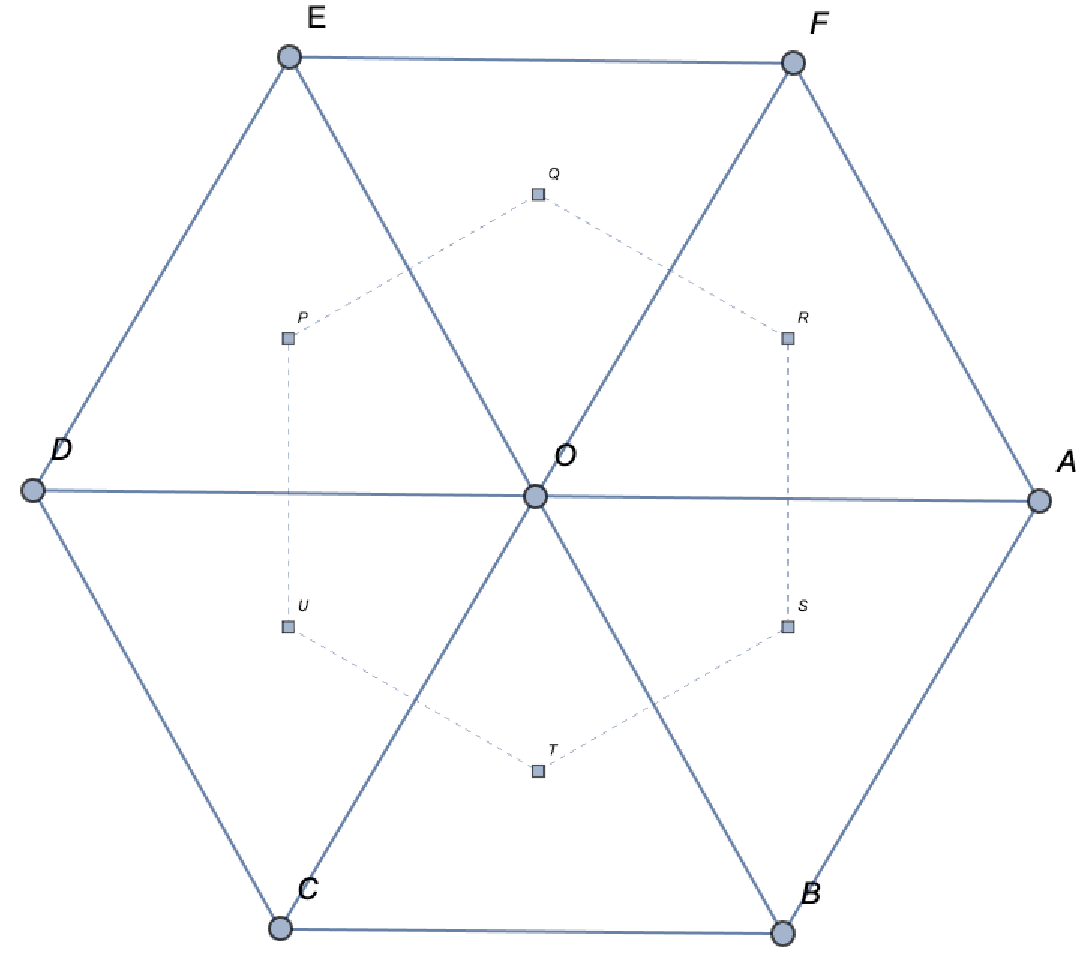
\includegraphics[scale=0.5]{figs/dual_graph.pdf}
    \end{center}

    \item
    $\star_0\alpha_0$ is a dual 2-form.\\
    $\star_1\alpha_1$ is a dual 1-form.\\
    $\star_2\alpha_2$ is a dual 0-form.\\

    \item
    We will use the barycentric dual for vertices which is $\ifrac13 \sum\text{(triangle area)}$ where we sum over surrounding triangles.\\
    The vertices of the dual graph lie on the centroids, which we will use later.\\
    $A,B,C,D,E,F$ have 2 surrounding triangles. $O$ has 6. 
    \begin{align}
        (\star_0\alpha_0)(v^\star) &:= |\text{Area}(v^\star)|\alpha_0(v) \nt\\\nt\\
        (\star_0\alpha_0)(A^\star) &= 2 \times \frac13 \frac{\sqrt3}{4} \times 1 = \frac{1}{2 \sqrt{3}} \nt\\
        (\star_0\alpha_0)(B^\star) &= 2 \times \frac13 \frac{\sqrt3}{4} \times 2 = \frac{1}{\sqrt{3}} \nt\\
        (\star_0\alpha_0)(C^\star) &= 2 \times \frac13 \frac{\sqrt3}{4} \times 3 = \frac{\sqrt{3}}{2} \nt\\
        (\star_0\alpha_0)(D^\star) &= 2 \times \frac13 \frac{\sqrt3}{4} \times 4 = \frac{2}{\sqrt{3}} \nt\\
        (\star_0\alpha_0)(E^\star) &= 2 \times \frac13 \frac{\sqrt3}{4} \times 5 = \frac{5}{2 \sqrt{3}} \nt\\
        (\star_0\alpha_0)(F^\star) &= 2 \times \frac13 \frac{\sqrt3}{4} \times 6 = \sqrt{3} \nt\\
        (\star_0\alpha_0)(O^\star) &= 6 \times \frac13 \frac{\sqrt3}{4} \times 7 = \frac{7 \sqrt{3}}{2} \nt
    \end{align}

    \item 
    \begin{wrapfigure}{r}{0.2\textwidth} %this figure will be at the right
        \centering
        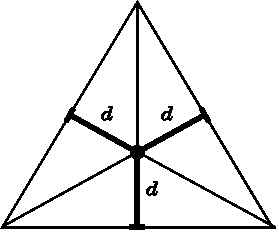
\includegraphics[width=0.2\textwidth]{figs/dual_edge.pdf}
    \end{wrapfigure}
    We will say that length of boundary dual edges is zero, so we only consider edges fanning out of vertex $O$.
    Height $h$ of an equilateral triangle: $1^2 = h^2 + \hal^2 \implies h = \ifrac{\sqrt3}{2}$. 
    Boxed here is Viviani's theorem [\href{https://en.wikipedia.org/wiki/Viviani%27s_theorem}{1}][\href{https://www.google.com/url?sa=t&rct=j&q=&esrc=s&source=web&cd=&cad=rja&uact=8&ved=2ahUKEwjqvLnXps35AhXbGVkFHUDADcYQFnoECA0QAw&url=https%3A%2F%2Fwww.maa.org%2Fsites%2Fdefault%2Ffiles%2FChen-CMJ-2006.pdf&usg=AOvVaw0kXL5NnMvqD5_oh29f4N_H}{2}]
    which states that:
    \begin{mdframed}
    Inside an equilateral
    triangle, the sum of the perpendicular distances from a point $P$ to the three sides is independent
    of the position of $P$ (and so equals the altitude of the triangle).
    \end{mdframed}
    If $P$ is the centroid, it would be exactly centered in the triangle, positioned equidistant to the sides.
    So, if $d$ is the distance to the sides, we have: $$3d = \ifrac{\sqrt3}{2} \implies d = \frac{1}{2\sqrt3}$$
    By symmetry, we argue that the edges of our dual graph all have length $2d = \ifrac{1}{\sqrt3}$.

    \begin{align}
        (\star_1\alpha_1)(e^\star) &:= \frac{|\text{Length}(e^\star)|}{|\text{Length}(e)|}\alpha_1(e) = \frac{\alpha_1(e)}{\sqrt3}\nt\\\nt\\
        (\star_1\alpha_1)((O,A)^\star) &= \frac{-2}{\sqrt3} \nt\\
        (\star_1\alpha_1)((O,B)^\star) &= \frac{-5}{\sqrt3} \nt\\
        (\star_1\alpha_1)((O,C)^\star) &= -\sqrt3 \nt\\
        (\star_1\alpha_1)((O,D)^\star) &= \frac{1}{\sqrt3} \nt\\
        (\star_1\alpha_1)((O,E)^\star) &= \sqrt3 \nt\\
        (\star_1\alpha_1)((O,F)^\star) &= \frac{-2}{\sqrt3} \nt
    \end{align}

    \item
    \begin{align}
        (\star_2\alpha_2)(f^\star) &:= \frac{\alpha_2(f)}{|\text{Area}( f )|} = \frac{4}{\sqrt3}\alpha_2(f)\nt\\
        (\star_2\alpha_2)((A,B,O)^\star) &= 4 \sqrt{3} \nt\\
        (\star_2\alpha_2)((C,B,O)^\star) &= -\frac{8}{\sqrt{3}} \nt\\
        (\star_2\alpha_2)((D,C,O)^\star) &= \frac{4}{\sqrt{3}} \nt\\
        (\star_2\alpha_2)((D,E,O)^\star) &= 0 \nt\\
        (\star_2\alpha_2)((E,F,O)^\star) &= -\frac{4}{\sqrt{3}} \nt\\
        (\star_2\alpha_2)((A,F,O)^\star) &= -\frac{8}{\sqrt{3}} \nt
    \end{align}

    \item
    Using the diagonal Hodge star from the lectures.
    For each edge $ij$, with halfedge $\alpha_{ij}$ and its twin $\eta(\alpha_{ij}) = \beta_{ij}$:
    $$
        \star_1 = \text{diag}\Bigl\{
            \begin{cases}
                \hal (\cot\alpha_{ij} + \cot\beta_{ij}), \quad \text{if $ij \notin$ boundary} \\
                0, \quad \text{if $ij \in$ boundary}
            \end{cases}
        \Bigr\}
    $$

    \item
    For each face $ijk$:
    $$
        \star_2 = \text{diag}\Bigl\{\frac{1}{A_{ijk}}\Bigr\}
    $$
\end{enumerate}



\end{document}
